\section{Introduction}\label{sec:intro}
The behavior of a programming language is fundamentally shaped by its semantics. It is essential to have a clear and well-defined semantics of a programming language. A precise and unambiguous definition of language semantics is the foundation upon which all subsequent development and analysis of the language rely. Without it, the language’s behavior becomes unpredictable and unmanageable.

Two primary approaches are commonly used to define the language semantics:
\begin{itemize}
\item \textbf{Declarative semantics} focuses on specifying the language’s behavior through formal, mathematical rules. It rigorously defines a high-level, abstract model of the language semantics, without delving into implementation details. Declarative semantics is often employed in theoretical contexts, such as academic research and formal verification, to reason about language properties like type soundness.
\inred{(story about interactive theorem provers…?)}
\item \textbf{Algorithmic semantics} utilizes detailed, stepwise instructions, usually presented in pseudocode, to define the language behavior. It offers a concrete, implementation-oriented view of how the language should be executed. ECMAScript adopts this approach to describe the semantics of JavaScript with abstract algorithms in well-structured English sentences.
\end{itemize}

While language semantics can be specified \textit{manually} with paper and pencil, there are approaches to \textit{mechanize} the semantics definitions. These mechanization techniques provide a structured representation of language semantics. In some instances, they go a step further, enabling the semantics to be executable. The choice of mechanization method critically depends on the specific style of semantics utilized in the language specification.

For declarative-style semantics, general-purpose language frameworks such as PLT-Redex and the K framework have been developed. PLT-Redex specializes in actuating the rewrite rules with evaluation contexts. The K framework defines K rules, their specialized abstraction over rewrite rules, to specify and execute language semantics.
\inred{(use cases of the two frameworks)}

Algorithmic-style semantics, as exemplified in ECMAScript, find mechanization in the ESMeta toolchain. ESMeta parses the structured English sentences and translates them into an internal representation, IRES. IRES has its own semantics, and thereby can be executed with an interpreter implementation. Executing the JavaScript semantics in IRES allows an indirect execution of JavaScript programs.
\inred{(how it led to JEST, JSTAR, JSAVER, …)}
Notably, ESMeta has been gracefully integrated into the continuous integration (CI) system of ECMAScript as of 2022.

\begin{figure}[t]
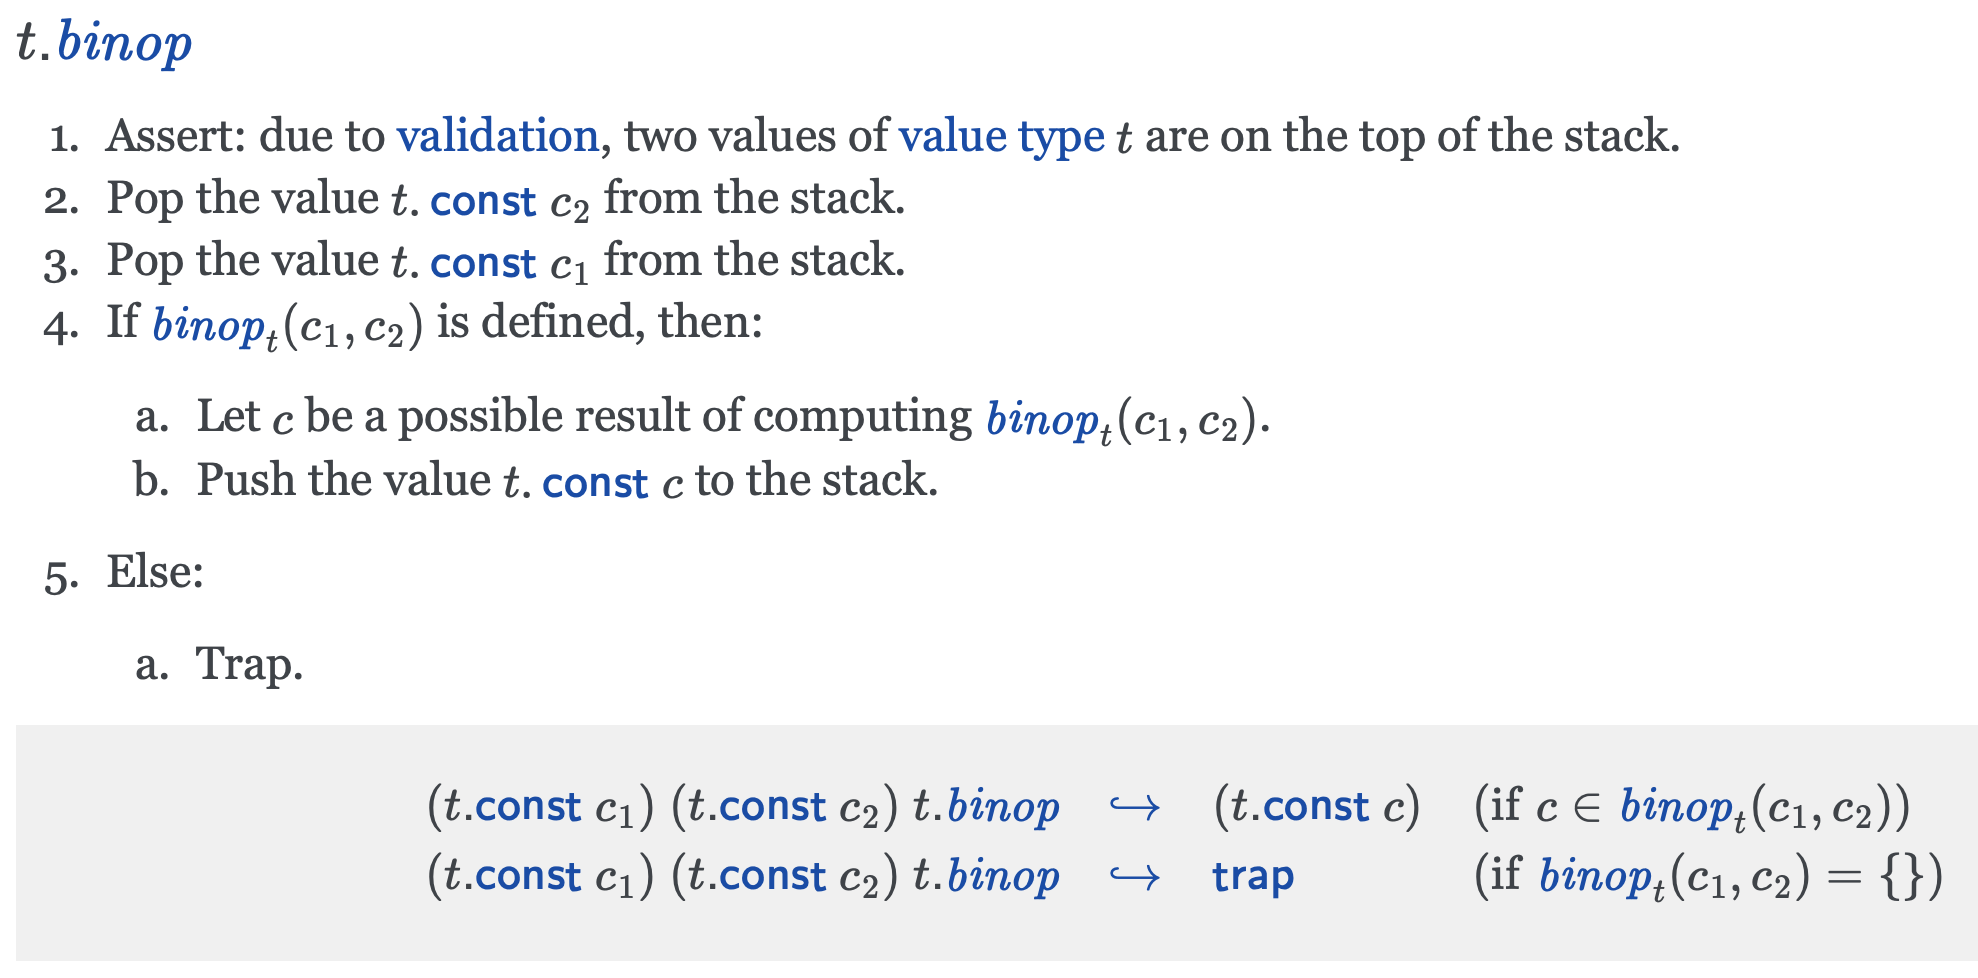
\includegraphics[width=.7\textwidth]{../img/spec.png}
\caption{The binary operator semantics in the specification}
\label{fig:spec}
\end{figure}

WebAssembly, commonly referred to as Wasm, takes advantage of the two worlds, blending both declarative and algorithmic styles to define its semantics. For example, Figure~\ref{fig:spec} is the execution semantics of the Wasm $t.\mbox{\emph{binop}}$ binary operator instruction from the official specification. Figure~\ref{fig:spec}(a) presents the 
\textit{prose pseudocode} description of the $t.\mbox{\emph{binop}}$ instruction. It breaks down the execution of the instruction into five sequential steps. Figure~\ref{fig:spec}(b) below specifies the operational semantics in rewrite rules. The two styles cater to the dual needs of spec writers and readers. Prose serves for the comprehension of spec readers, typically engine developers. Rewrite rules serve the needs of language designers, whose interests are the clarity and correctness of the language semantics. The two complementary forms of semantics must be equivalent in terms of the behavior being specified.

Despite its sophisticated nature of presenting the dual semantics, every piece of the Wasm specification thus far has been manually written. This poor authorship support introduces several challenges in preparing and maintaining the Wasm specification text:
\begin{itemize}
\item \textbf{Properly typesetting the specification is a tedious and labor-intensive task.}
 Both representations must be typesetted in LaTeX for the formal notations and in reStructuredText for the prose pseudocode. Although it generates human-friendly pdf, HTML documents, the source file itself lacks visual clarity.
\inred{(quotes from spec authors)}
\item \textbf{Manual processes are susceptible to human error, potentially leading to inconsistencies or inaccuracies in the specification.}
The dual semantics representation opens the door to a wide range of errors.
\inred{Rewrite rules may contain an error. Prose pseudocode may contain an error. Synchronization between the two styles can also be a challenge. (elaborate on each types of error)}
\item \textbf{Maintaining a manual specification becomes increasingly challenging as Wasm evolves.} Wasm is a growing language, continually accepting proposals to add features. After its initial release in 2017 as version 1.0, several proposals, including SIMD, were merged into the official specification in 2022, bumping up to version 2.0. Currently, proposals including Garbage Collected Types, Threads, and Exception Handling are being developed to comprise Wasm 3.0. Manual efforts will surely hinder the growth of Wasm in the face of future proposals.
\end{itemize}

\begin{figure}[t]
\footnotesize
\begin{verbatim}
rule Step_pure/binop-val:
  (CONST nt c_1) (CONST nt c_2) (BINOP nt binop) ~> (CONST nt c)
  -- if $binop(binop, nt, c_1, c_2) = c

rule Step_pure/binop-trap:
  (CONST nt c_1) (CONST nt c_2) (BINOP nt binop) ~> TRAP
  -- if $binop(binop, nt, c_1, c_2) = epsilon
\end{verbatim}
\caption{The binary operator semantics in SpecTec DSL}
\label{fig:dsl}
\end{figure}

To address these challenges, we introduce \textbf{SpecTec}, a tailored language framework that mechanizes the Wasm specification process. SpecTec defines
a \emph{Domain-Specific Language (DSL)}, to succinctly describe the syntax, type system, and the execution semantics of Wasm. In contrast to the official specification, SpecTec’s DSL deliberately and exclusively chooses declarative style to document the execution semantics. Figure~\ref{fig:dsl} illustrates the semantics of $t.\mbox{\emph{binop}}$ instruction in the DSL. Its close resemblance to the formal notations in the official specification envisions a straightforward way of automatically typesetting the DSL into LaTeX. Put another way, SpecTec accepts language specification in its DSL as input and produces a typesetted LaTeX document as output. In such a process, SpecTec analyzes the semantic definitions to identify inconsistencies such as typos and arity mismatches.

Most interestingly, we have devised a mechanism to automatically derive the algorithmic prose from the declarative rewrite rules written in the DSL. The declarative rules can indeed stand as a single source of truth, as it contains necessary information to be translated into an algorithmic format. We identify that the transformation is actually a NP-hard problem, and propose a novel solution. The generated prose can easily be pretty-printed in reStructuredText format. Together with the automatically generated LaTeX file of the formal notation, they readily comprise the complete specification document.

The automatic generation of algorithmic prose even facilitates the execution of Wasm semantics. The algorithmic prose is structured in AL, our language designed to express the Wasm semantics. Coupled with an AL interpreter, this approach allows for indirect execution of Wasm programs. This has enabled us to test our generated algorithmic semantics against the Wasm official test, giving evidence that the algorithmic semantics align with the intended behavior outlined in the original declarative semantics.

In summary, our contribution is \textbf{SpecTec}, a comprehensive toolchain for the Wasm specification:
\begin{itemize}
\item \textbf{SpecTec allows language designers to concisely specify the syntax and semantics of Wasm.} SpecTec explicitly separates the concern of language design and documentation. No other effort than to specify the syntax and semantics in SpecTec DSL is necessary, as SpecTec automatically typesets the definitions in LaTeX.
\item \textbf{SpecTec builds a bridge from declarative style semantics to algorithmic style semantics.} Defining the declarative style semantics as a single source of truth, SpecTec automatically generates an equivalent version in an algorithmic style. This significantly lessens the burden for spec authors.
\item \textbf{SpecTec provides meta-level error checking in the process of writing the specification.} The formal semantics in DSL can be checked for typos or arity mismatches. An automatic generation of the corresponding algorithmic semantics ensures consistency in the prose throughout the specification document. Moreover, we have tested that the generated prose preserves the intentions in the formal rewrite rules.
\inred{(test pass rate 100\%?)}
\item \textbf{SpecTec is a forward-compatible toolchain that can adapt to the evolving Wasm semantics.} We showcase the application of SpecTec to an upcoming proposal \inred{Exception Handling}. 
\end{itemize}

Our goal is to integrate SpecTec toolchain into the Wasm standardization process in the near future, ensuring a more efficient and reliable path for defining and evolving Wasm semantics.
